\documentclass[conference]{IEEEtran}
\IEEEoverridecommandlockouts

% Packages
\usepackage{cite}
\usepackage{amsmath,amssymb,amsfonts}
\usepackage[dvipsnames]{xcolor}
\usepackage{graphicx}
\usepackage{textcomp}
\usepackage{listings}
\usepackage{subcaption}
\usepackage{multirow}
\usepackage{algorithm}
\usepackage{algpseudocode}
\usepackage{algorithmicx}
\usepackage{url}
\usepackage{caption}
\usepackage{tcolorbox}
\usepackage{hyperref}
\usepackage[T1]{fontenc}
\usepackage{enumitem}
\usepackage{multicol}
\usepackage{enumitem}
\usepackage{balance}

\setlength {\marginparwidth }{2cm}

\hypersetup{hidelinks}
\newcommand{\algorithmautorefname}{Algorithm}
\captionsetup[algorithm]{name=Alg.} 

\tcbuselibrary{listingsutf8}
\newtcbox{\redbox}[1][]{
 on line, 
 boxsep=1pt, 
 left=1pt, 
 right=1pt, 
 top=1pt, 
 bottom=1pt, 
 colframe=red!75!black, 
 colback=red!10, 
 boxrule=0.5pt, 
 rounded corners,
 #1
}

\algrenewcommand\algorithmicindent{0.8em} 

\hyphenation{GROMACS}
\hyphenation{LAMMPS}
\hyphenation{ls1 mardyn}
\hyphenation{AutoPas}


\begin{document}

\title{Auto-Tuning with Early Stopping in AutoPas}

\author{
    \IEEEauthorblockN{ Manuel Lerchner}
    \IEEEauthorblockA{
        \textit{Technical University of Munich}\\
        Munich, Germany}
}

\maketitle

\begin{abstract}
    Simulating molecular dynamics (MD) presents a significant computational challenge due to the vast number of particles involved in modern experiments. Naturally, researchers have put much effort into developing algorithms and frameworks that can efficiently simulate these systems. This paper focuses on the AutoPas framework, a modern particle simulation library that uses dynamic optimization techniques to achieve high performance in complex simulation scenarios. We introduce the AutoPas framework and investigate a possible improvement to AutoPas' auto-tuning capabilities by introducing an early stopping mechanism aiming to reduce the overhead of parameter space exploration. Our evaluation shows that such a mechanism can reduce the total simulation time by up to 21.1\% in specific scenarios, demonstrating the potential of this improvement.
\end{abstract}

\begin{IEEEkeywords}
    molecular dynamics, auto-tuning, AutoPas, early-stopping, GROMACS, LAMMPS, ls1 mardyn
\end{IEEEkeywords}

\section{Introduction}

Molecular dynamics simulations represent a computational cornerstone in various scientific fields. These simulations typically use complex and computationally intensive interaction models acting on enormous numbers of particles to ensure accurate results. Consequently, the computational requirements for these simulations can be substantial and require highly optimized algorithms and frameworks to achieve feasible performance.

Well-established molecular dynamics engines, such as GROMACS, LAMMPS, and ls1 mardyn, solve this challenge by providing a single, highly optimized implementation determined before the start of the simulation. As their implementation is determined statically, these engines must rely on static optimizations to improve their performance. Static optimizations are typically selected based on predefined performance models and must be fine-tuned for specific hardware architectures. Common static optimization techniques include automatic optimizations performed by modern compilers (e.g., loop unrolling, inlining, auto-vectorization), conditional compilation based on the target hardware (e.g., SIMD), or manual selection of simulation parameters based on expert knowledge~\cite{Gratl2019AutoPas}.

AutoPas approaches the challenge of high-performance molecular dynamics simulations differently: Instead of choosing a single implementation prior to the simulation, AutoPas uses dynamic optimizations to adjust its implementation based on the simulation state and the actual hardware performance. This approach is favorable, as the engine can adapt and optimize itself without external intervention. However, dynamic optimizations come at the cost of increased complexity and potential overhead due to the need for frequent re-evaluations of the selected implementation.

This paper provides an overview of the AutoPas framework and the benefits and challenges of using dynamic auto-tuning in molecular dynamics simulations. Moreover, we investigate the potential of an early stopping mechanism and evaluate its performance in the context of the AutoPas framework.

\section{Related Work}

Established MD engines such as GROMACS, LAMMPS, and ls1 mardyn have been developed over many years and have been optimized to achieve high performance in their respective use cases. This section provides an overview of the default implementations of these engines.

\subsection{GROMACS}

GROMACS implements a single, highly optimized variant of the Verlet Cluster List algorithm. The algorithm allows for flexible cluster sizes specifically designed for achieving good SIMD vectorization~\cite{PALL20132641}.

Gromacs allows setting the vectorization parameters for the cluster size $M$ and the number of particles in neighbor groups $N$ statically to tune the force calculations to the SIMD width of the system~\cite{PALL20132641}. With suitable values for $M$ and $N$, computations of $M \times N$ particle interactions can be performed with just two SIMD load instructions~\cite{Solving_Software_Challenges_Exascale_2014}, drastically reducing the number of memory operations required for the force calculations and reaching up to 50\% of the peak flop rate on all supported hardware platforms~\cite{Solving_Software_Challenges_Exascale_2014}.

Tuning those parameters is time-consuming and relies on a detailed understanding of many low-level software optimization aspects of the different hardware platforms~\cite{PALL20132641}. In GROMACS, the developers must create and maintain such performance models for each supported hardware platform, which is a time-consuming and labor-intensive process~\cite{PALL20132641}.

\subsection{LAMMPS}

LAMMPS utilizes a performance-optimized version of the Verlet List algorithm. To optimize cache performance, LAMMPS stores its neighbor lists in a global data structure split across multiple memory pages. Each page stores neighbor lists for multiple particles in a contiguous memory block, allowing for efficient allocation and deallocation of the neighbor lists~\cite{THOMPSON2022108171}. All particle data is stored in a Structure of Arrays (SoA) layout~\cite{THOMPSON2022108171}, allowing for efficient vectorization of the force calculations.

\subsection{ls1 mardyn}

ls1 mardyn differs from the previously mentioned MD engines as it uses the Linked Cells algorithm for particle interactions. Using LinkedCells provides a better memory efficiency than GROMACS and LAMMPS, allowing for simulations of massive particle systems~\cite{tchipev2019twe}. Internally, ls1 mardyn uses the default data layout of \textit{AoS} (Array of Structures) for storing particle data and converts it to an \textit{SoA} (Structure of Arrays) layout when required. Particular branches aimed at simulating massive particle systems can use a \texttt{RMM} (Reduced Memory Mode) layout, allowing for simulations of up to twenty trillion atoms~\cite{tchipev2019twe}.

\vspace{0.2cm}

While GROMACS, LAMMPS, and ls1 mardyn achieve remarkable performance through specialized and statically optimized implementations, their reliance on manual tuning and hardware-specific adjustments presents challenges. These limitations have led to the development of frameworks like AutoPas, which aim to dynamically optimize their performance based on the simulation state and hardware characteristics.

\section{AutoPas}

AutoPas\footnotemark\ was developed on the basis of creating an efficient node-level particle simulation engine applicable to a wide range of scientific fields~\cite{Tchipev2020}. To achieve this goal, AutoPas uses a modular architecture that seamlessly integrates different algorithms and data structures into the simulation engine. As it is not capable of running simulations on its own, AutoPas serves as an intermediary layer between user-provided simulation code and implementations specifically designed to efficiently solve N-Body problems. The modular nature of AutoPas enables it to combine different implementations and create a wide range of so-called \textit{configurations}.

To eliminate the need for manual configuration selection and enable dynamic optimization, AutoPas provides an auto-tuning framework. This framework periodically assesses different configurations and selects optimal ones based on performance metrics. This selection process is managed by \textit{TuningStrategies} that systematically suggest promising configurations to evaluate. \autoref{fig_architecture} illustrates the high-level architecture of the AutoPas library.

\begin{figure}[H]
    \centering
    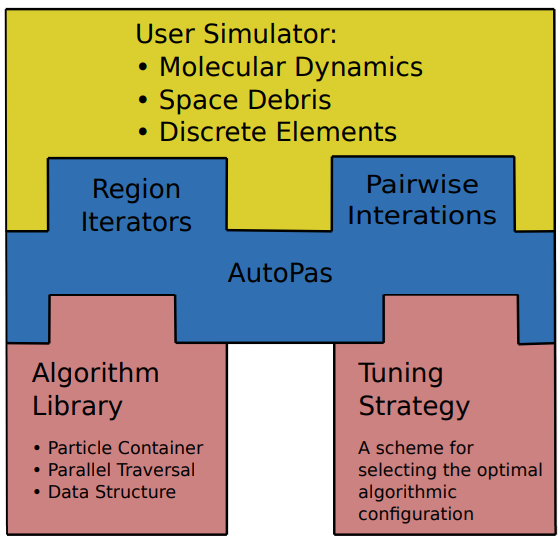
\includegraphics[width=1.9in]{figures/AutoPasLibraryStructure.png}
    \caption{AutoPas Library Structure as depicted by~\cite{Newcome2023Poster}}
    \label{fig_architecture}
\end{figure}

\subsection{Algorithm Library}

\footnotetext{\label{fn:autopas}\href{https://github.com/AutoPas/AutoPas}{
        https://github.com/AutoPas/AutoPas}}


All different algorithmic implementations for solving N-Body problems are part of the so-called \textit{Algorithm Library} of AutoPas. The Algorithm Library contains different implementations for certain key aspects of the simulation, such as neighbor identification, traversal patterns, memory layouts, and optimization techniques. Currently, AutoPas supports the six tunable parameters: \textit{Container}, \textit{Data Layout}, \textit{Newton 3}, \textit{Traversal}, \textit{Load Estimator} and \textit{Cell Size Factor} which can be combined to create different configurations.

Maintaining a library of different implementations has several benefits: As the library is modular, it is straightforward to add new, potentially hardware-specific, implementations for each key aspect of the simulation. This ensures that the simulation engine remains maintainable and can provide performance portability across a wide range of hardware platforms. The interchangeable nature of the implementations also ensures implicit backward compatibility, making it easy to study the effects of new hardware on existing implementations. Users of the library also benefit from this approach. As AutoPas is able to automatically select the best configuration for their specific use case and hardware setup, users do not need to have a deep understanding of the underlying hardware or software optimizations and can fully focus on the high-level aspects of their simulation~\cite{Tchipev2020}\cite{Gratl2022AutoPas}.

\subsection{Tunable Parameters}

This section provides a brief overview of the six tunable parameters available in AutoPas.

\begin{description}[style=nextline]
    \item[Container]
        Containers are responsible for storing the simulation particles so that relevant neighbor particles can be determined efficiently. As AutoPas focuses on short-range interactions with a force cutoff radius $r_c$, efficient neighbor identifications using just $O(N)$ distance calculations are possible~\cite{Gratl2019AutoPas}. The container types depicted in \autoref{fig_containers} will be shortly described below.

        \begin{description}[style=nextline, font=\itshape]
            \item[$\bullet$ Linked Cells]
                The Linked Cells algorithm maintains a grid of cells, each storing a list of particles located within the cell. When calculating forces for a particle, only\footnote{If $cellSizeFactor = {cellSize}/{r_c} = 1$.} particles in neighboring cells (depicted in blue) must be considered, as all other particles are guaranteed to be outside the cutoff radius.

                LinkedCells introduces many spurious distance calculations (shown by arrows to gray particles), which can be reduced by using a smaller cell size factor~\cite{menges2019}. LinkedCells are very cache-friendly as spatially close particles are stored together in memory~\cite{Gratl2022AutoPas}.

            \item[$\bullet$ Verlet Lists]
                The Verlet Lists algorithm uses a second radius $r_v = {r_c} + \Delta_s$ (yellow circle) and considers all particles within this radius as potential neighbors. Contrary to LinkedCells, each particle maintains its own list of potential neighbors, resulting in a higher memory overhead.
                As the bigger radius $r_v$ provides a buffer region, it is possible to only rebuild the neighbor-list every $n$ simulation steps, as long as no particle can move from outside $r_c + \Delta_s$ to inside $r_c$ unnoticed~\cite{NEWCOME2023115278}.

                VerletLists have few spurious distance calculations but are less cache-friendly as neighboring particles are not stored together in memory~\cite{Gratl2022AutoPas}. This results in very inefficient vectorization~\cite{PALL20132641}.

            \item[$\bullet$ Verlet Cluster Lists]
                The Verlet Cluster Lists algorithm improves on the VerletLists algorithm by grouping particles into clusters of size $M$ ($M=4$ in the figure) and performing neighbor-list calculations on a cluster level~\cite{PALL20132641}. This reduces the memory overhead significantly. However, it results in more spurious distance calculations as all particles in neighboring clusters must be considered when calculating forces. When $M$ is chosen in accordance with the SIMD width of the system, efficient vectorization is possible~\cite{Gratl2022AutoPas}~\cite{PALL20132641}.
        \end{description}

        \begin{figure}[h]
            \centering
            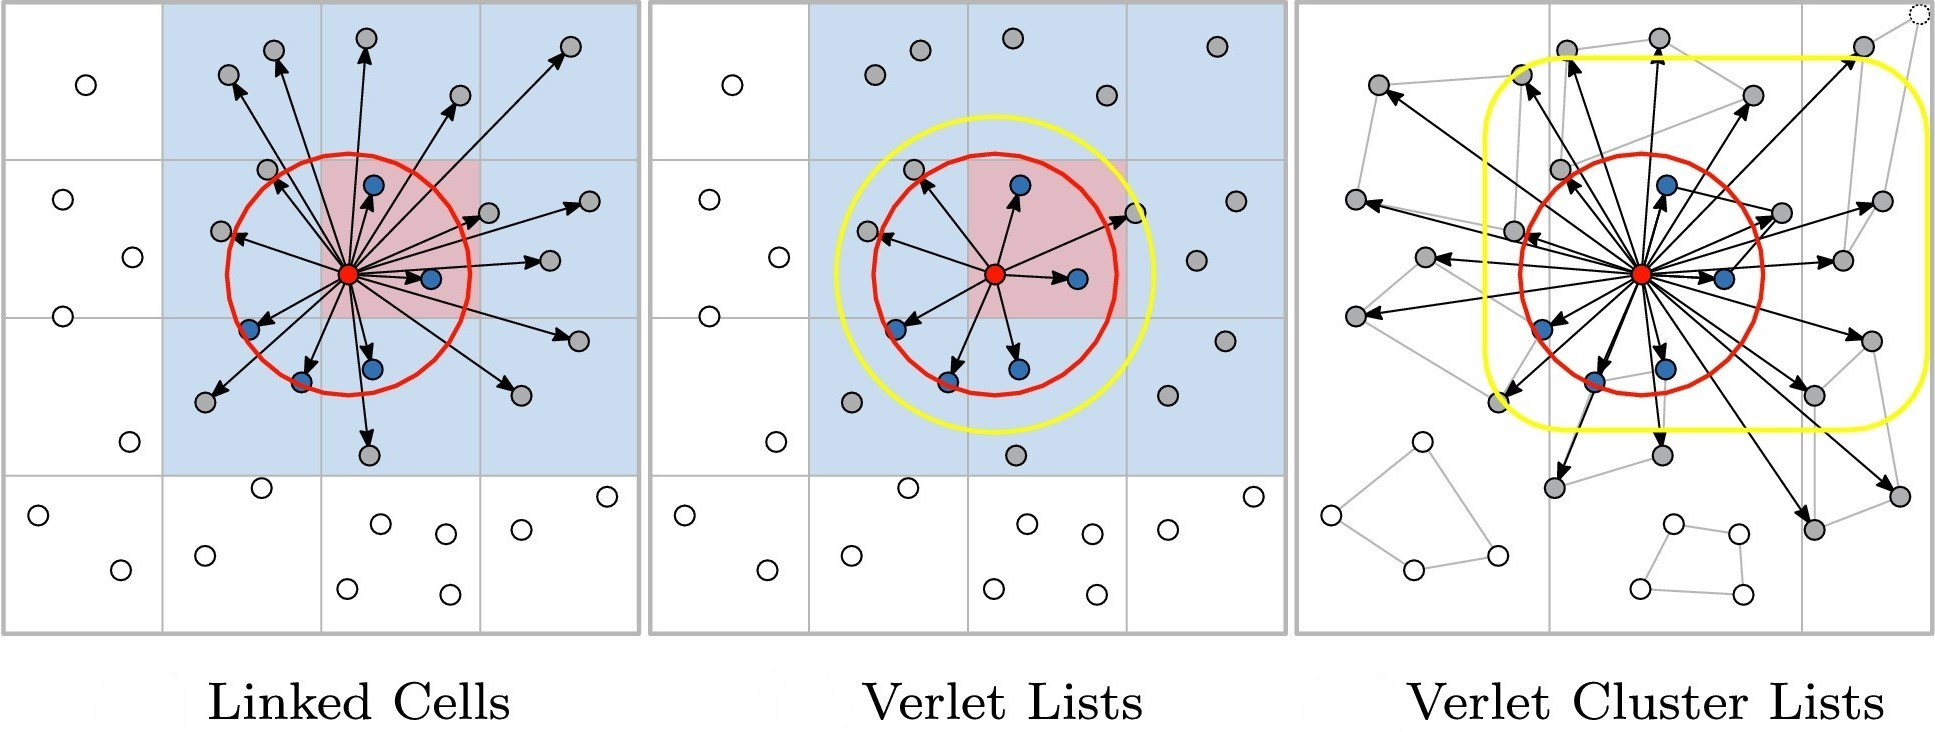
\includegraphics[width=\columnwidth]{figures/containers.jpg}
            \caption{Important container types as depited by~\cite{Gratl2022AutoPas}. The cutoff radius $r_c$ is shown using a red circle. Arrows represent distance checks between particles. Only particles shown in blue contribute to the final force calculation.}
            \label{fig_containers}
        \end{figure}

    \item[Data Layout]
        The Data Layout describes how the particles are stored in memory. Possible choices are \textit{SoA} (Structure of Arrays) and \textit{AoS} (Array of Structures). \textit{SoA} allows for better vectorization as properties of multiple particles can be loaded efficiently into SIMD registers. However, accessing the properties of a single particle is more expensive, requiring
        multiple memory accesses. \textit{AoS} is the opposite. It allows for efficient access to properties of a single particle to, e.g., send it to another MPI rank, but results in inefficient vectorization~\cite{Gratl2022AutoPas}.

    \item[Newton 3]
        A common optimization in molecular dynamics involves applying Newton's third law to reuse force calculations between particle pairs, effectively reducing computational costs by half. However, not all parallel traversal patterns can safely implement this optimization without risking race conditions. For those that do, synchronization points must be added to ensure accurate force application, which in turn limits the potential for parallelism.

    \item[Traversal]
        Traversals are responsible for iterating over the particles in the simulation and calculating their interactions in a shared-memory environment~\cite{SECKLER2021101296}. The traversal pattern determines to which extent force calculations can be parallelized and whether optimizations, such as Newton 3, can be applied. The traversal patterns depicted in \autoref{fig_traversals} will again be shortly introduced below.

        \begin{description}[style=nextline, font=\itshape\mdseries]
            \item[$\bullet$ C01]
                The C01 traversal pattern processes each cell independently, resulting in an embarrassingly parallel traversal. Newton's Third Law cannot be used with this traversal pattern since adjacent cells are processed simultaneously, which could lead to race conditions when applying forces. As no synchronization between cells is required, the C01 traversal pattern has the highest degree of parallelism~\cite{NEWCOME2023115278}.
            \item[$\bullet$ C18]
                The C18 traversal pattern uses color assignments to ensure that no race conditions occur when using Newton 3. \autoref{fig_traversals} shows the regular color assignments, ensuring that no two cells of the same color share common neighbors. To ensure that forces are only applied once when using Newton 3, each cell only applies forces to cells \textit{above} or \textit{right} of it. During the force calculation, all available threads work on a single color, which allows for a safe application of forces on neighboring cells and reduces scheduling overhead~\cite{NEWCOME2023115278}. As the color groups must be processed sequentially, the C18 traversal introduces 18 synchronization points, which reduces the overall degree of parallelism\cite{NEWCOME2023115278}.

            \item[$\bullet$ C08]
                The C08 traversal pattern is similar to the C18 traversal pattern but uses a different coloring scheme with only eight colors, reducing the number of synchronization points to eight. The C08 traversal pattern has a degree of parallelism between the C01 and C18 traversal patterns~\cite{NEWCOME2023115278}.
        \end{description}

        \begin{figure}[H]
            \centering
            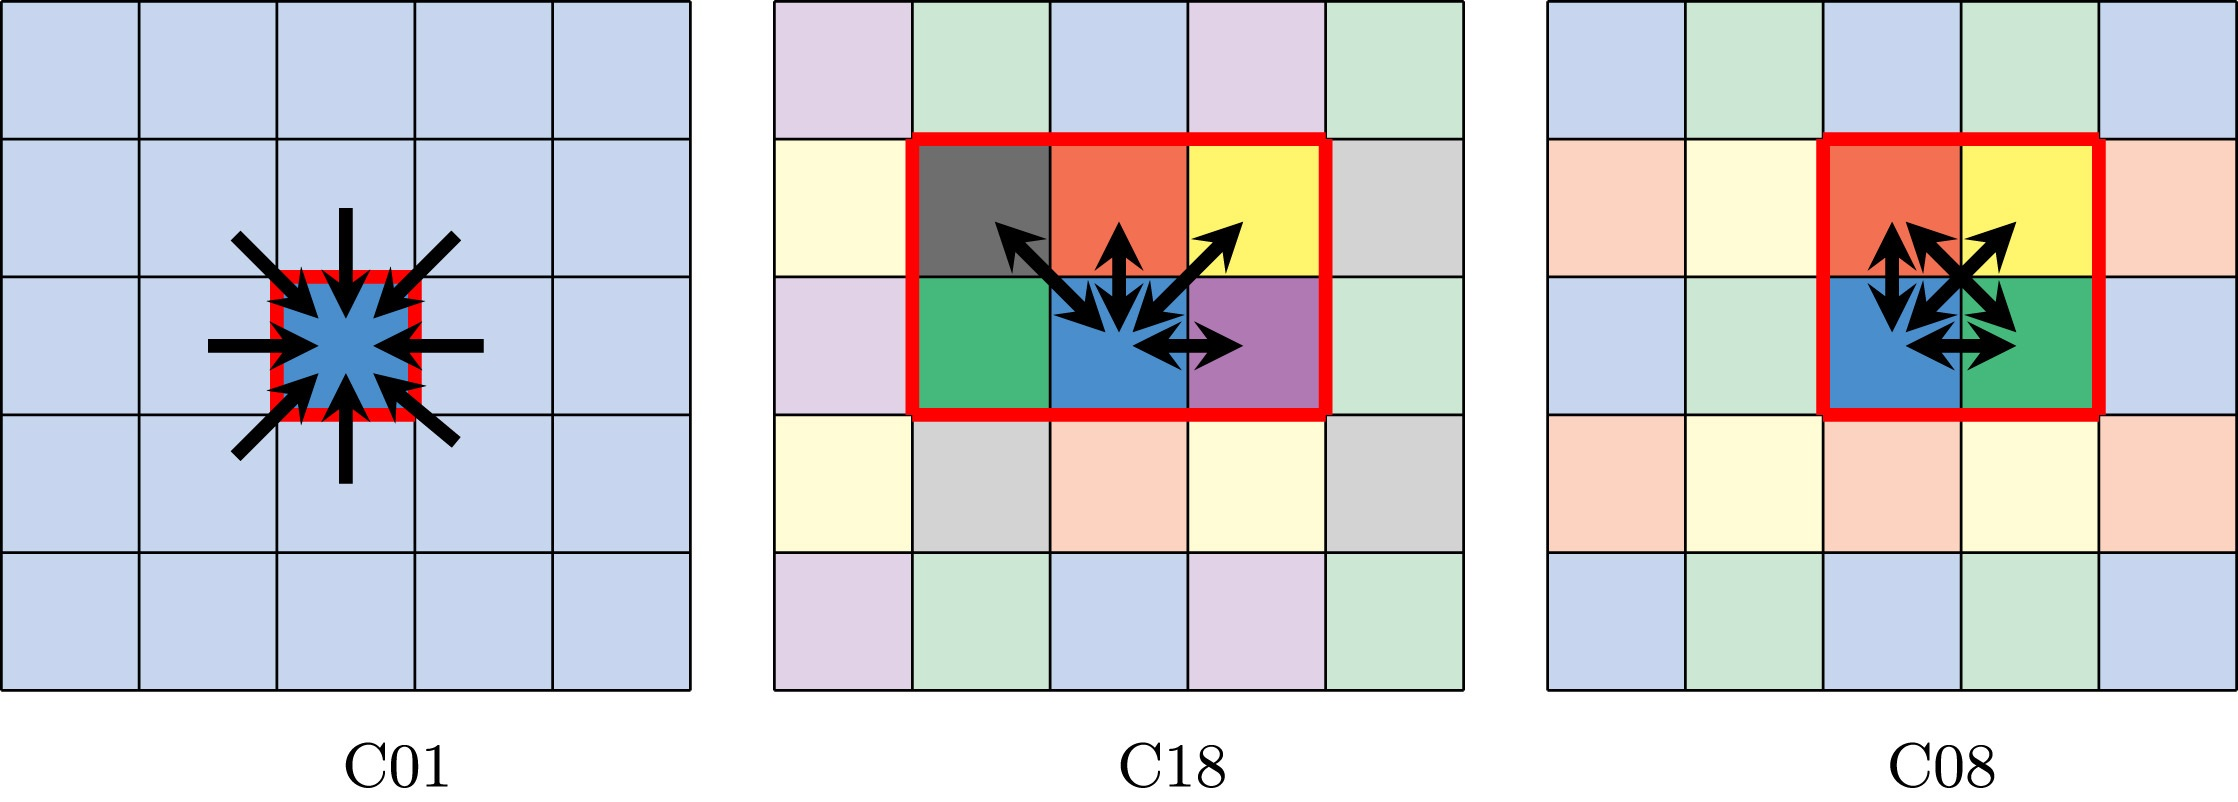
\includegraphics[width=\columnwidth]{figures/traversals.jpg}
            \caption{Important Traversal Types as depicted by~\cite{NEWCOME2023115278}.}
            \label{fig_traversals}
        \end{figure}

    \item[Load Estimator]
        Different load estimators can be used to estimate and fairly divide work across all available processing units. Maintaining a good workload distribution reduces the idle time of processing units and thus increases the overall simulation speed.

    \item[Cell Size Factor]
        The default cell size factor of 1 results in a cell size of $r_c$ (see \autoref{fig_containers}). As discussed previously, the large area of neighboring cells causes many spurious distance calculations, which can be reduced by using a smaller cell size factor. As decreasing the cell size factor also increases the memory overhead due to the higher number of cells to be maintained in memory~\cite{menges2019}~\cite{Papula2020}, the cell size factor must be chosen carefully.
\end{description}


\subsection{Auto-Tuning Framework}

A manual selection of suitable implementations for each tunable parameter would require extensive domain knowledge that is challenging to acquire and maintain under the constantly changing software and hardware landscape. To address this issue, AutoPas performs automated algorithm selection to optimize specific performance metrics, such as runtime or energy efficiency~\cite{Gratl2022AutoPas}. Internally, AutoPas periodically initiates so-called \textit{tuning-phases} in which promising configurations are evaluated in order to determine the best configuration for the current simulation state. The winning configuration is then used until the next tuning phase is initiated.

The currently available tuning strategies in AutoPas are:

\begin{description}[style=nextline]
    \item[FullSearch]
        The FullSearch strategy naively evaluates all possible configurations, thus always finding the best configuration.

    \item[RandomSearch]
        The RandomSearch strategy randomly selects configurations out of the entire search space, causing less overhead than the FullSearch strategy at the cost of potentially missing the best configuration.

    \item[BayesianSearch]
        The Bayesian Search strategy is similar to the RandomSearch strategy. However, it uses a Bayesian optimization algorithm to select the next configuration to evaluate based on previous measurements~\cite{njan_master}. An improvement to better account for the discrete tuning space of AutoPas called \textit{BayesianClusterSearch} is also available~\cite{njan_master}.

    \item[PredictiveTuning]
        The PredictiveTuning strategy extrapolates previously gathered timing measurements of a configuration to predict its performance in the current simulation state. This allows for an efficient rejection of inefficient configurations without evaluating them~\cite{pelloth2020}.

    \item[RuleBasedTuning]
        The RuleBasedTuning strategy uses a set of rules to discard undesirable configurations immediately. The rules are based on expert knowledge in a \textit{if-then} fashion and use aggregate statistics of the simulation state to make decisions~\cite{endreport.pdf}.

    \item[FuzzyTuning]
        The FuzzyTuning strategy is similar to the RuleBasedTuning strategy but uses fuzzy logic systems to evaluate configurations. This allows for both an inter- and extrapolation of the rules to account for configurations not covered by the expert knowledge~\cite{Manuel_Lerchner_Thesis.pdf}.

\end{description}

\section{Benefits of Auto-Tuning}

Since no single configuration can deliver optimal performance across all simulation scenarios~\cite{Tchipev2020}, dynamic performance tuning is essential for maintaining high efficiency across diverse simulation conditions. This section discusses some of the key benefits of using AutoPas's auto-tuning framework.

\subsection*{Performance Improvements}

The most compelling advantage of auto-tuning is the significant performance improvements it can achieve. It has been shown many times that AutoPas can improve simulation times across diverse molecular dynamics simulation scenarios, both in the standalone application as well as in established MD engines such as ls1 mardyn and LAMMPS~\cite{SECKLER2021101296}\cite{Gratl2022AutoPas}. Those improvements provide compelling evidence for the effectiveness and importance of the auto-tuning approach.

\subsection*{Accessibility and Ease of Use}

AutoPas's tuning framework enables users to achieve optimal performance directly out of the box without requiring deep expertise in performance optimization. Different performance characteristics caused by varying hardware setups are automatically accounted for by the auto-tuning framework, allowing users to focus on the actual simulation~\cite{Tchipev2020}.

The inherent user-friendliness is particularly valuable when integrating AutoPas into other simulation frameworks, as developers can treat the simulation engine as a black box and let the auto-tuning framework handle the optimization.

\section{Drawbacks of Auto-Tuning}

\subsection*{Suboptimal Configurations}

A major drawback of auto-tuning in the way it is implemented in AutoPas is the inherent overhead caused by tuning phases. Even though it is an important characteristic of tuning strategies to infer and evaluate only those configurations that are likely to perform well, this inference is not always successful. Many configurations can turn out to be orders of magnitude slower than the optimal configuration~\cite{endreport.pdf}\cite{Manuel_Lerchner_Thesis.pdf}, making their evaluation extremely costly.

Advanced tuning strategies such as \textit{RuleBasedTuning} or \textit{FuzzyTuning} can mitigate this problem to some extent, however even they cannot guarantee always finding the best configuration, as the underlying expert knowledge for both strategies is expected to be highly incomplete.

This challenge highlights the need for additional optimization techniques, such as the early stopping mechanism introduced in \autoref{sec:early-stopping}, to reduce the overhead caused by evaluating suboptimal configurations.

\autoref{fig:unnecessary-tuning-phases} shows a typical timing profile of the ExplodingLiquid simulation for every available tuning strategy. The inherent overhead caused by tuning phases is very noticeable and is present in all tuning strategies. For some tuning strategies, the overhead results in a considerable increase in the total simulation time (see default cases in \autoref{fig:full_search} and \autoref{fig:predictive_tuning}).

\subsection*{Periodic Re-Tuning}

Even though AutoPas is capable of performing periodic auto-tuning, it is often beneficial to just execute a single tuning phase right at the beginning of the simulation.

Ideally, the aforementioned overhead of evaluating suboptimal configurations leads to discovering a better configuration at the end of the tuning phase. However, many scenarios, especially homogeneous ones with simple interaction models, tend to behave fairly stable over time, making it very likely that re-tuning does not lead to an improved configuration. In such cases, the overhead of re-tuning is unnecessary and only increases the total simulation time. \autoref{fig:unnecessary-tuning-phases} depicts this effect for the ExplodingLiquid simulation.

Further evaluation of the data obtained in \cite{lerchner2024} shows that only three out of 184 runs using slight variations of example scenarios provided by \texttt{md-flexible}\footnote{
    \texttt{md-flexible} is a molecular dynamics simulation framework making use of the AutoPas library. It is included in the AutoPas repository and provides a wide range of example scenarios to demonstrate the capabilities of the AutoPas library.
} show any changes in the best configuration after the initial tuning phase. This effect occurs in both single and multi-node simulations and indicates that all currently provided example scenarios of \texttt{md-flexible} are incapable of demonstrating the benefits of periodic re-tuning.

More complex scenarios, most likely involving multiple MPI ranks and inhomogeneous particle distributions, are necessary to fully demonstrate the benefits of periodic re-tuning. Simulating such inhomogeneous scenarios in an MPI environment increases the chance of varying particle distribution across both MPI ranks and time steps, increasing the likelihood of benefitting from periodic re-tuning on each rank (See \cite{Newcome2023Poster}).

\begin{figure}[h]
    \centering
    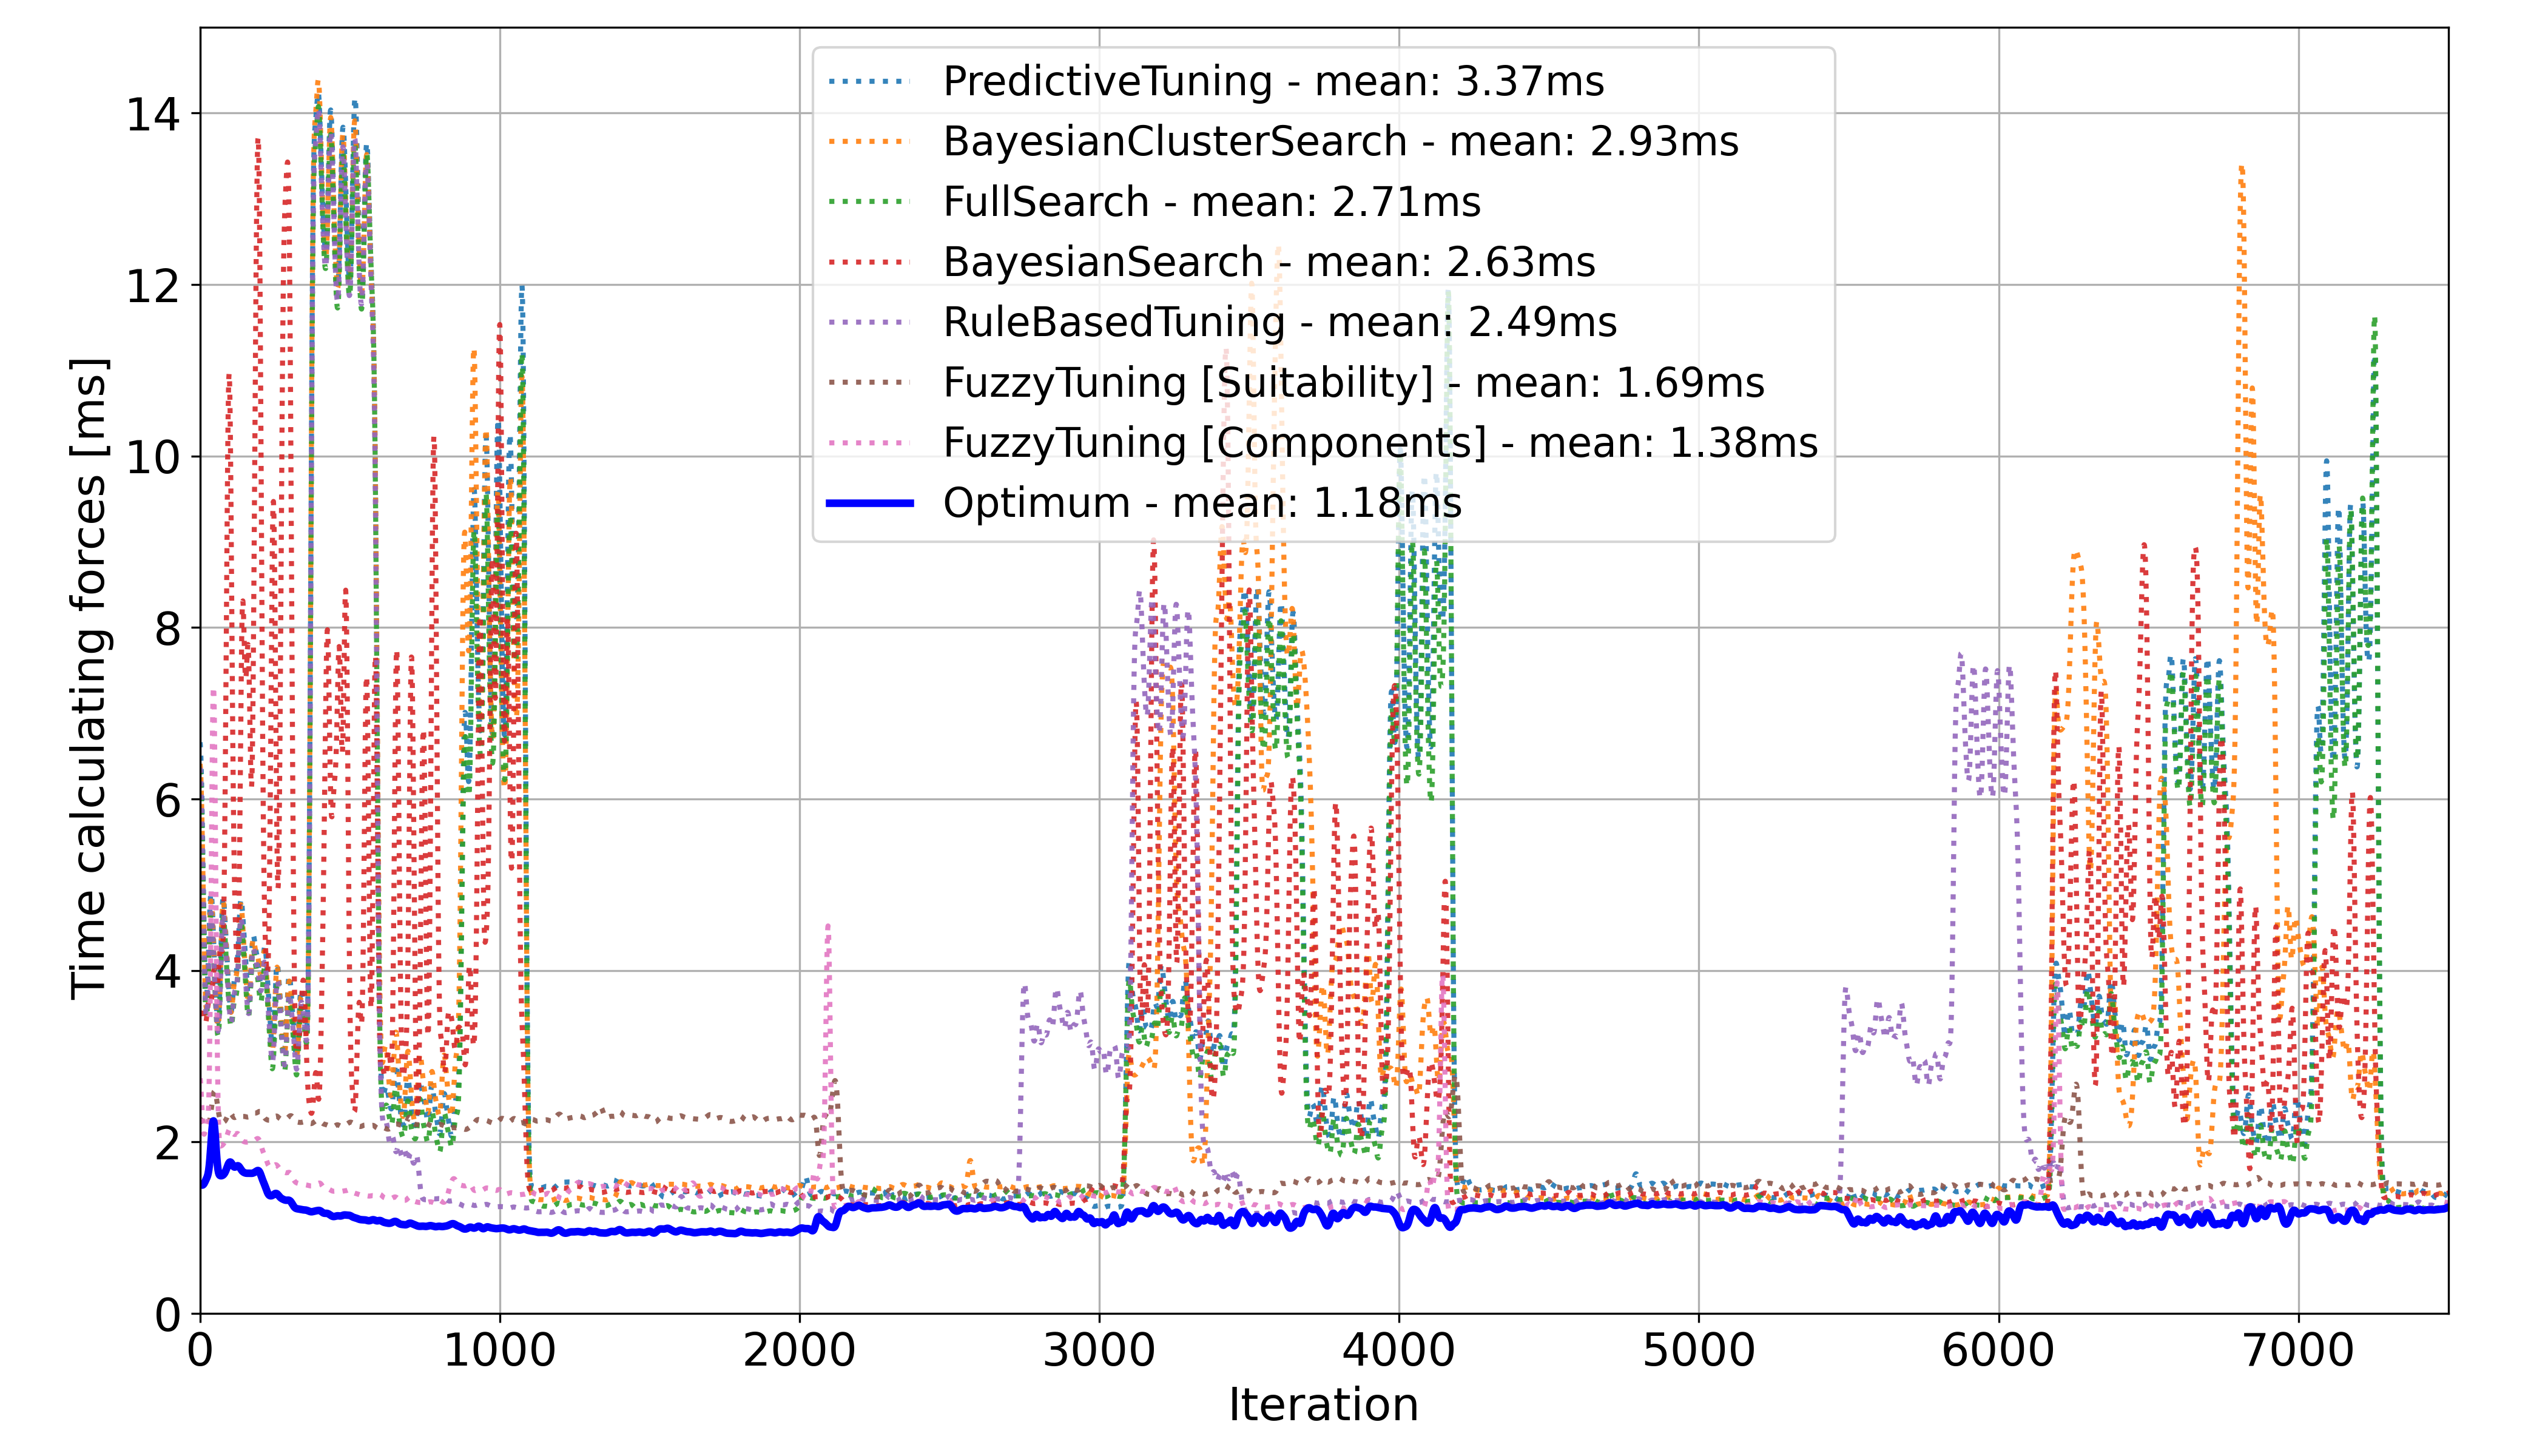
\includegraphics[width=\columnwidth]{figures/unnecessary-tuning-phases.png}
    \caption{
        Typical timing profile of the ExplodingLiquid simulation for every available tuning strategy. The plot clearly shows that all tuning strategies introduce overhead during the tuning phases. Data obtained from \cite{lerchner2024}
    }
    \label{fig:unnecessary-tuning-phases}
\end{figure}

\newpage

\section{Early Stopping Optimization}
\label{sec:early-stopping}

To minimize some of the introduced drawbacks of the auto-tuning process, \cite{endreport.pdf}\cite{Manuel_Lerchner_Thesis.pdf}\cite{autopas_issue673} suggest that an \textit{early stopping} mechanism could be beneficial for the AutoPas framework. The primary goal of such a mechanism would be to detect tuning iterations that take much longer than the currently best-known configuration and to stop the evaluation of those configurations early. There are two approaches to this problem:


\begin{itemize}
    \item \textbf{Stopping Further Samples}\\
          As AutoPas evaluates a configuration multiple times to reduce measurement noise, a simple way to implement early stopping would be to stop the evaluation of further samples as soon as it is clear that the performance is significantly worse than the best-known configuration. This approach however requires fully evaluating some samples of a bad configuration.
    \item \textbf{Interrupting the Evaluation}\\
          A more fine-grained approach, proposed in~\cite{endreport.pdf}, could interrupt the evaluation of a long-running configuration while it is still being evaluated. Such a change would require a big rewrite of AutoPas' internal structure and is therefore not feasible in the short term.
\end{itemize}

To get a first impression of the potential benefits of an early stopping mechanism, we implemented the first approach into the AutoPas framework\footnote{
    See \href{https://github.com/AutoPas/AutoPas/pull/995}{
        https://github.com/AutoPas/AutoPas/pull/995} for the changes.
}. The changes to the existing codebase are minimal, as the early-stopping mechanism can be implemented using existing functionality. \autoref{alg_early_stopping} shows the main changes to the \texttt{AutoTuner.cpp} file.

Both described approaches require a user-defined threshold, called $earlyStoppingFactor$, to determine how much slower a configuration can be compared to the best-known configuration before it should be stopped early. The effect of this threshold will be evaluated in the following section.

\begin{algorithm}[h]
    \small
    \caption{Early Stopping Algorithm in AutoPas}
    \label{alg_early_stopping}
    \begin{algorithmic}[1]
        \Procedure{checkEarlyStoppingCondition}{~}
        \If{not $\Call{enoughConfidence}{~}$}
        \State \Return
        \EndIf
        \State $evidenceEstimate \gets \Call{estimateRuntimeFromSamples}{~}$
        \State $bestEvidence \gets \Call{getLatestOptimalConfiguration}{~}$
        \State $slowdownFactor \gets \frac{evidenceEstimate}{bestEvidence}$
        \If{$slowdownFactor > earlyStoppingFactor$}
        \State $abort \gets true$
        \EndIf
        \EndProcedure

        \vspace{0.2em}

        \Procedure{GetNextConfiguration}{}
        \If{not $inTuningPhase$}
        \State \Return ($currentConfig, false)$
            \ElsIf{$numSamples$ $<$ $maxSamples$ \redbox{\textbf{and} not $abort$}}
            \State \Return $(currentConfig, true)$
            \Else
            \State $stillTuning \gets \Call{tuneConfiguration}{~}$
            \State \Return $(newConfig, stillTuning)$
        \EndIf
        \EndProcedure
    \end{algorithmic}
\end{algorithm}

\subsection{Evaluation: Exploding Liquid Simulation}
\label{sec:evaluation}

To evaluate the performance of the early stopping mechanism, we perform benchmarks using the Exploding Liquid scenario\footnote{
    The input file can be found at \href{
        https://github.com/AutoPas/AutoPas/blob/master/examples/md-flexible/input/explodingLiquid.yaml}{explodingLiquid.yaml}.
    A video of the simulation is available at \url{https://youtu.be/u7TE5KiSQ08}.
} provided by \texttt{md-flexible}. All runs are performed using a single node of the \href{https://doku.lrz.de/coolmuc-4-1082337877.html}{CoolMUC4} supercomputer using two threads and are repeated five times.

\begin{description}[style=nextline]
    \item[FullSearch (\autoref{fig:full_search})]
        Early stopping combined with the FullSearch strategy, is able to reduce the total simulation time from 13.93 seconds to 10.99 seconds at $earlyStoppingFactor \approx1.05$. This corresponds to reducing the total simulation time by 21.1\%.
    \item[PredictiveTuning (\autoref{fig:predictive_tuning})]
        Early stopping combined with the PredictiveTuning strategy, is able to reduce the total simulation time from 15.86 seconds to 12.58 seconds at $earlyStoppingFactor \approx1.05$. This corresponds to reducing the total simulation time by 20.7\%.
    \item[FuzzyTuning (\autoref{fig:fuzzy_tuning})]
        Early stopping combined with the FuzzyTuning strategy shows no significant changes in the total simulation time.
\end{description}

\begin{figure}[h]
    \centering
    \begin{subfigure}[b]{\columnwidth}
        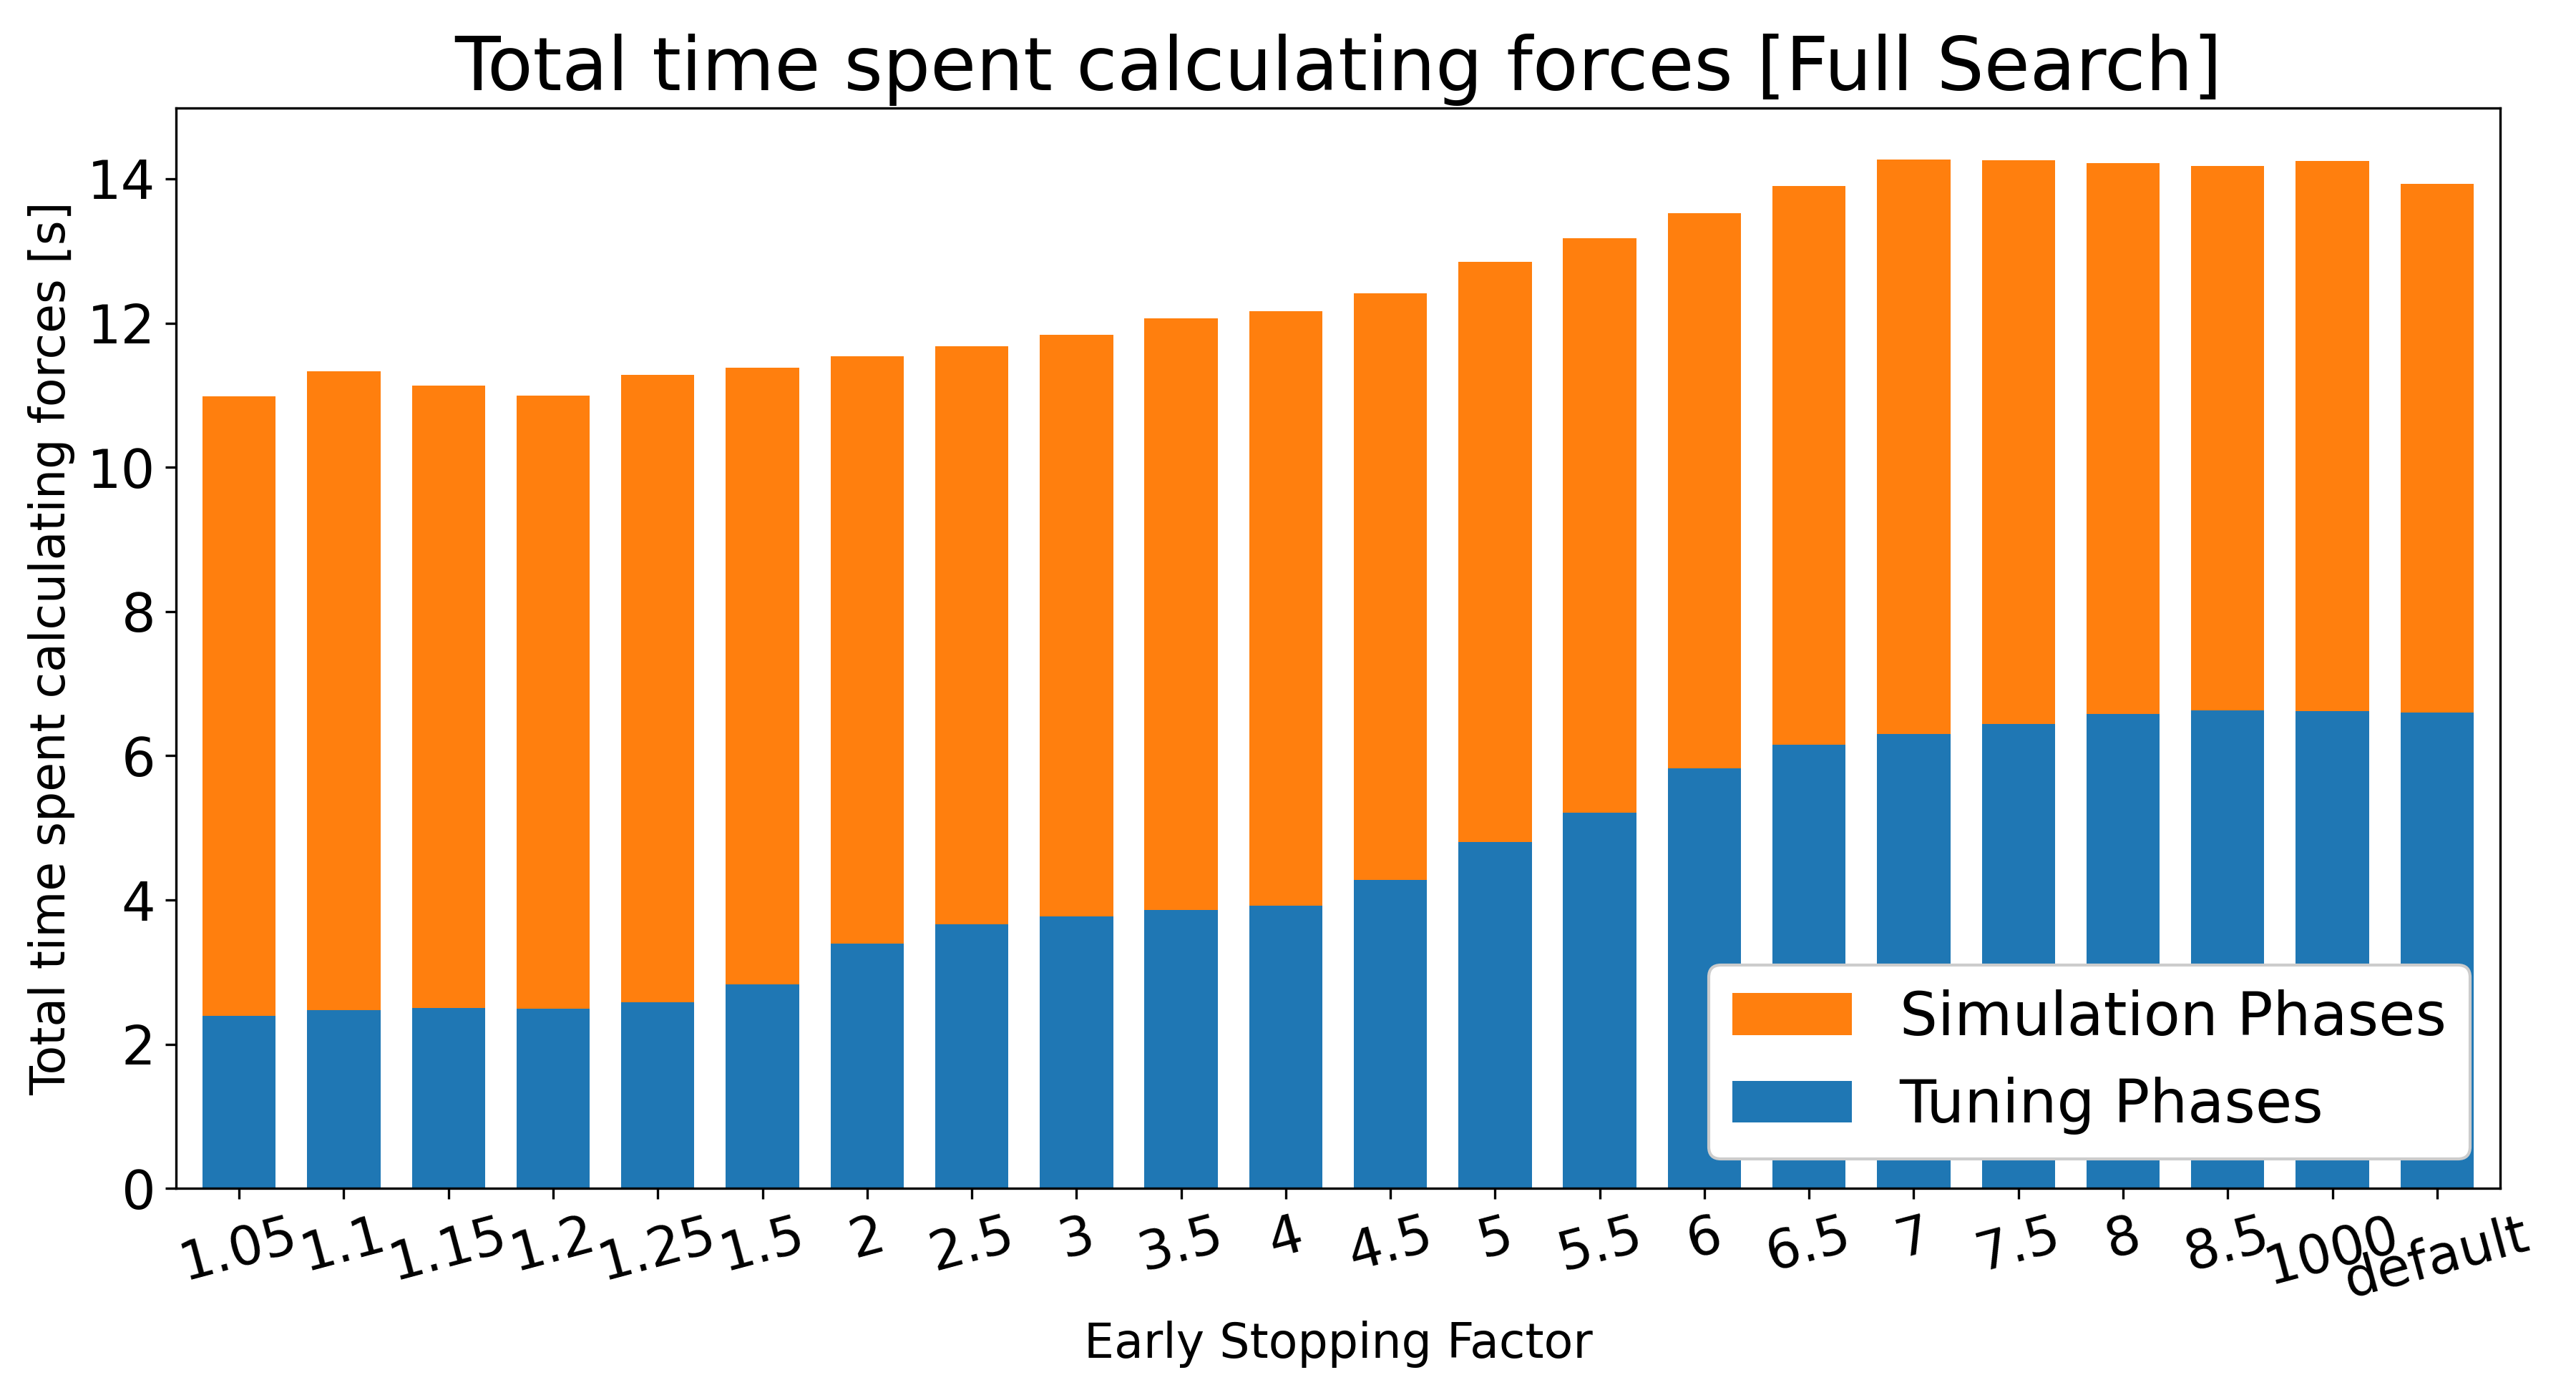
\includegraphics[width=\columnwidth]{../data/explodingLiquid/cluster/fullSearchEvidenceBased_2threads/analytics/total_time_average.png}

        \caption{Time spent calculating forces for Exploding Liquid Scenario using the FullSearch strategy with early stopping and two threads.}
        \label{fig:full_search}
    \end{subfigure}

    \begin{subfigure}[b]{\columnwidth}
        \centering

        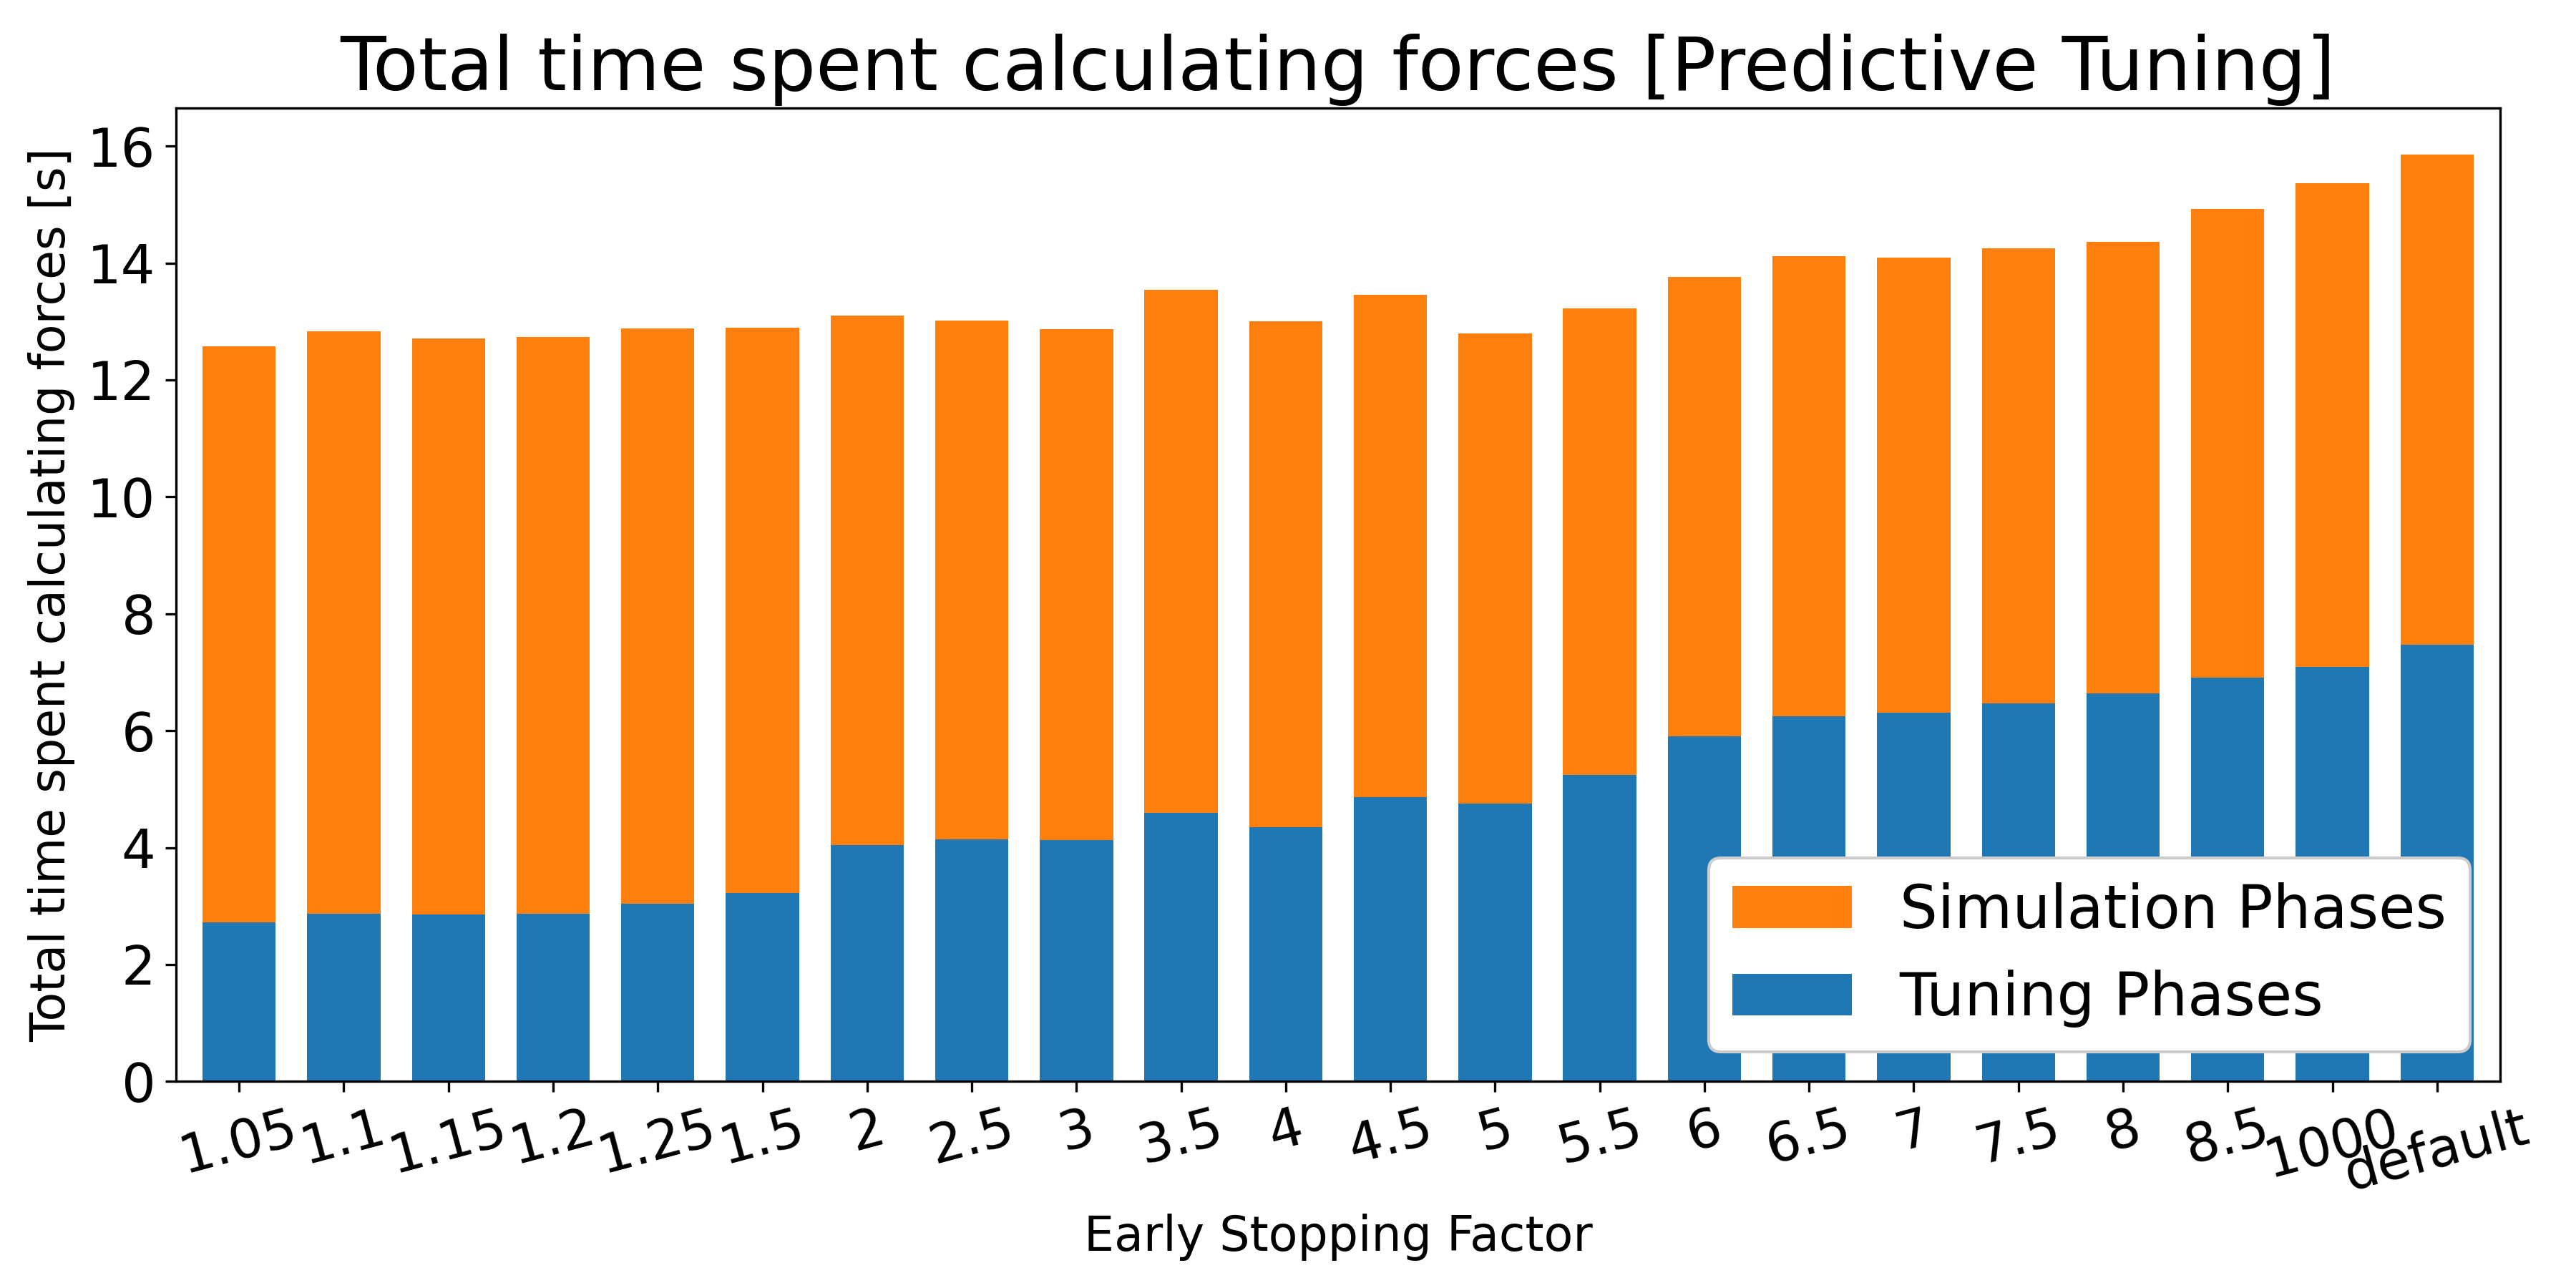
\includegraphics[width=\columnwidth]{../data/explodingLiquid/cluster/predictiveTuningEvidenceBased_2threads/analytics/total_time_average.png}

        \caption{Time spent calculating forces for Exploding Liquid Scenario using the PredictiveTuning strategy with early stopping and two threads.}
        \label{fig:predictive_tuning}
    \end{subfigure}

    \begin{subfigure}[b]{\columnwidth}
        \centering

        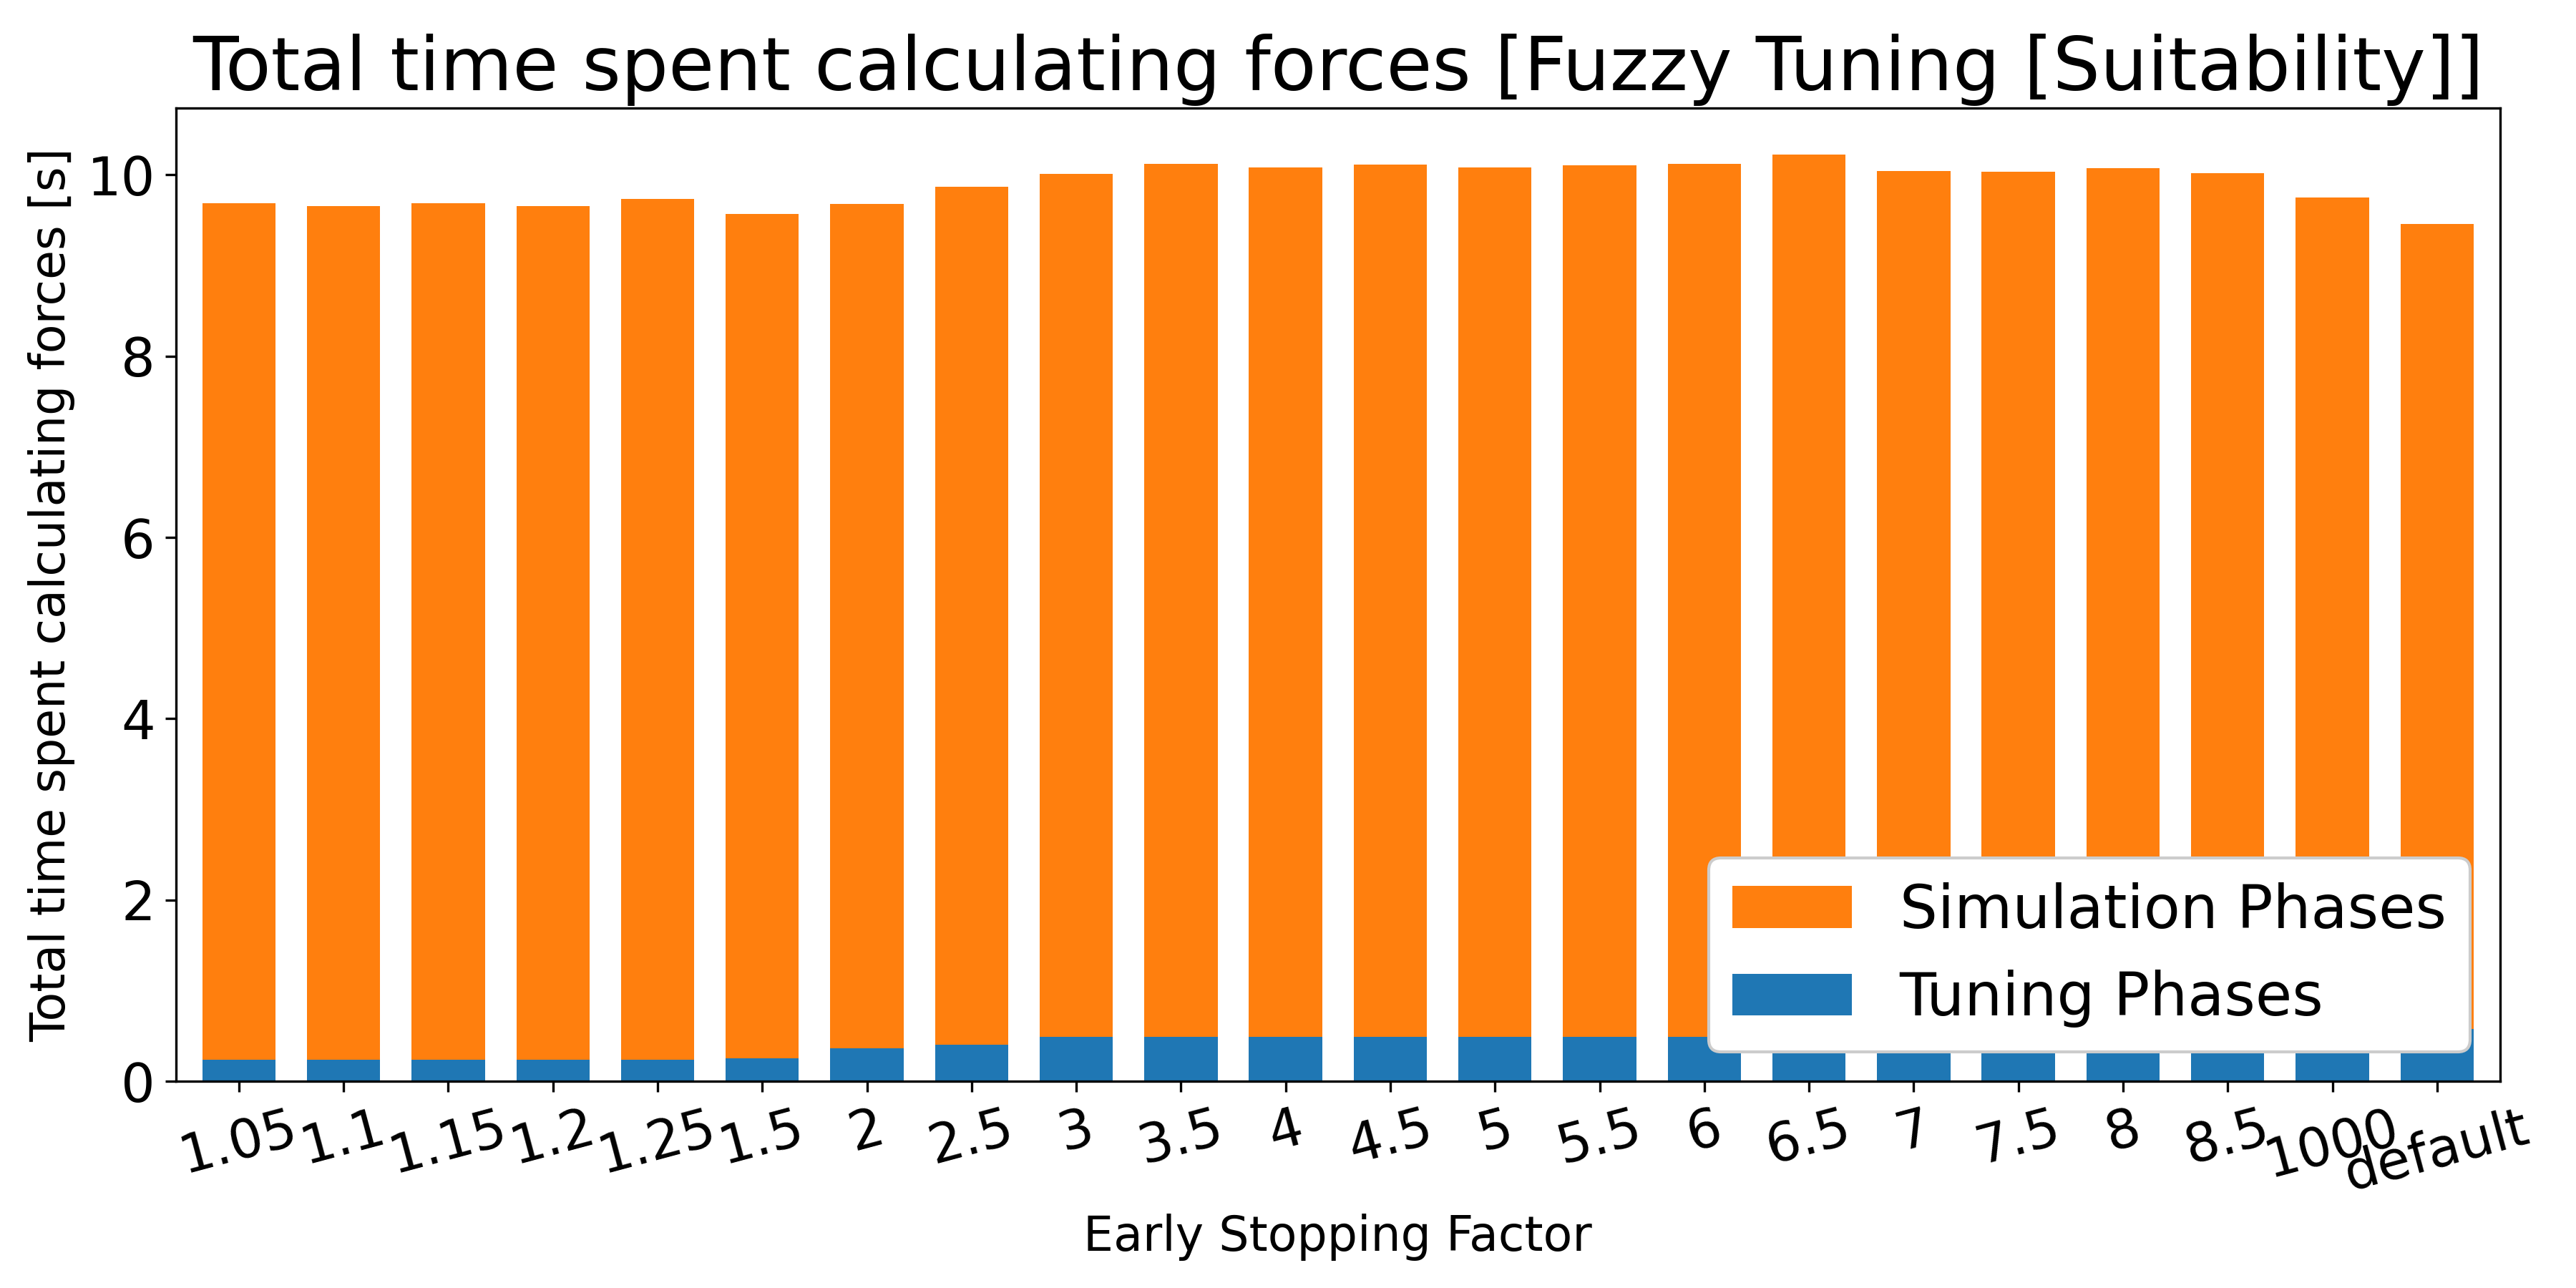
\includegraphics[width=\columnwidth]{../data/explodingLiquid/cluster/fuzzyTuningEvidenceBased_2threads/analytics/total_time_average.png}

        \caption{Time spent calculating forces for Exploding Liquid Scenario using the FuzzyTuning[Suitability] strategy with early stopping and two threads.}
        \label{fig:fuzzy_tuning}
    \end{subfigure}
\end{figure}

\subsection{Analysis and Discussion}
\begin{description}[leftmargin=1.2em, font=\itshape, style=nextline]
    \item[Impact of the Early Stopping Factor:]
        As expected, the benchmark results suggest that choosing a lower $earlyStoppingFactor$ generally results in shorter simulation times whenever \textit{bad} configurations are present during the tuning phases. Further analysis suggests that tuning phases result in equally performing configurations regardless of the chosen $earlyStoppingFactor$, indicating that all
        performance improvements are directly caused by faster tuning phases.

        As the limiting case of $earlyStoppingFactor \rightarrow \infty$ effectively disables the early stopping mechanism, the performance converges to the default implementation without early stopping.

        Interestingly, the limit $earlyStoppingFactor \rightarrow 1$ does not impact the total simulation time negatively. This indicates that \texttt{estimateRuntimeFromSamples()} provides a reliable estimate of the actual performance even with few samples and thus allows for very aggressive early stopping.

        In general, the $earlyStoppingFactor$ should however be chosen high enough to provide a sufficient margin to account for measurement noise, while being low enough to stop the evaluation of slow configurations effectively. Based on the benchmark results, $earlyStoppingFactor \approx 1.5$ seems to be a good compromise, as lower thresholds only provide marginal improvements.

        It is however unclear whether such a threshold is universally applicable to all scenarios. Additional benchmarking across a broader range of use cases is needed to validate these preliminary findings.

    \item[Impact of the Tuning Strategy:]
        The evaluated benchmarks show that the FullSearch and PredictiveTuning strategies benefit drastically from early stopping. As the FullSearch strategy naturally encounters many bad configurations, such a big improvement is expected. The PredictiveTuning strategy, on the other hand, is not able to leave the initial data collection phase, as the benchmark is too short. Longer benchmarks are needed to show the differences between FullSearch and PredictiveTuning more clearly.

        The FuzzyTuning strategy is unaffected by the early stopping mechanism, as it already performs nearly optimally without early stopping. This indicates that the FuzzyTuning strategy is very effective at avoiding bad configurations, making the early stopping mechanism redundant.

    \item[Future Work:]
        The current implementation of the early stopping mechanism starts with a fresh set of evidence samples in each tuning phase. This results in not using the information gathered in previous tuning phases, which could potentially help to stop evaluating bad configurations earlier. An improved version could keep track of a running average of evidence measurements collected during the prior simulation phase, allowing the early stopping mechanism to start with a reasonable estimate of achievable performance, thus increasing the likelihood of stopping more unsuitable configurations early.
\end{description}

\section{Conclusion}

We presented an overview of the AutoPas framework and its auto-tuning capabilities and demonstrated the benefits and challenges of dynamic auto-tuning in molecular dynamics simulations.

The main contribution of this paper is the introduction of an early stopping mechanism to reduce the overhead of parameter space exploration in the AutoPas framework. Our evaluation shows that such a mechanism can reduce the total simulation time by up to 21.1\% in specific scenarios with only minor changes to the existing codebase, demonstrating the potential of this improvement.

Further evaluation of the early stopping mechanism across a broader range of use cases is however necessary to validate these preliminary findings and to determine whether the early stopping mechanism is universally applicable to all scenarios.

\newpage

\bibliographystyle{IEEEtran}
\bibliography{literature}


\end{document}

